\documentclass{article}
\usepackage{graphicx}
\usepackage{graphics}
\usepackage[T1]{fontenc}
\usepackage[margin=1.2in]{geometry}
\usepackage{tcolorbox}
\usepackage{hyperref}
\usepackage{dingbat}
\usepackage{float}
\hypersetup{
    colorlinks=true, %set true if you want colored links
    linktoc=all,     %set to all if you want both sections and subsections
    linkcolor=blue,  %choose some color if you want links to stand out
    urlcolor=blue,
}
\begin{document}
\begin{titlepage}

\newgeometry{left=1.12in,right=1.12in,top=1in,bottom=1in}
\vspace{0.2in}

\begin{center}
\Large{\bf Statechart Based Modeling of Tasks and Code Generation}
\end{center}


\begin{center}

\vspace{15 mm}
{\it A Project Report \\
Submitted by}\\
\vspace{10mm}

\large{\bf Rohit Khuspe \\ \& \\ Mukesh Prajapati}
\\
\vspace{10mm}
 {\it Under the Mentorship of}
 \vspace{5mm}

 \large{\bf Naveen Cherupally} \\
\vspace{12 mm}
%\includegraphics[scale=0.3]{./figs/iitb_logo.jpg}
\vspace{10 mm}

\large{\bf Department of Computer Science \& Engineering} \\
\vspace{7mm}
\large{\bf Indian Institute of Technology, Bombay}
\end{center}

\end{titlepage}
\newpage
\pagenumbering{roman}
\tableofcontents
\newpage
%\section{Abstract}
%\section{Introduction}
\newpage
\listoffigures
\newpage
\pagenumbering{arabic}
\begin{abstract}
 Statecharts are one of the 5 UML diagrams which can be used to model the
dynamic behavior of the system.Statecharts are used to give abstract description of the behaviour of a system. This behaviour is analysed and represented as a series of events that can occurs in one or more possible state.
 It is highly desirable to represent any complex system with the
statecharts as they provide much abstraction
 which is very useful to implement a system. Writing the code manually for
building of any system includes lot
 of man power(resources) and prone to errors and most importantly consumes
much time. To make the task simple it is very
 desirable to auto-generate the code from the statecharts.  In this project we will be learning syntax and symantics of statecharts, how we can model a particular system or task using statecharts with the help of various tools.
 \end{abstract}
\newpage

\section{Introduction}
A Statechart is type of diagram used in Computer Science, Embedded systems and related field to describe the behaviour of system.Statecharts are used to give abstract description of the behaviour of a system. This behaviour is analysed and represented as a series of events that can occurs in one or more possible state.A statechart or statechart model consists of several components.The most important part is the state diagram, comprising states and transitions. They are organized into zero or more regions.The definition sections is a textual statechart component. It contains definitions of namespaces, interfaces, variables, events, operations, etc.
\newpage
\section{How Statechart diagrams are different from other state diagrams:}
Statechart diagrams are used to model dynamic aspect of a system like other state diagrams. But it has some distinguishing characteristics for modeling dynamic nature.\\
Statechart diagram defines the states of a component and these state changes are dynamic in nature. So its specific purpose is to define state changes triggered by events. Events are internal or external factors influencing the system.\\
Statechart diagrams are used to model states and also events operating on the system. When implementing a system it is very important to clarify different states of an object during its life time and statechart diagrams are used for this purpose. When these states and events are identified they are used to model it and these models are used during implementation of the system.\\
If we look into the practical implementation of Statechart diagram then it is mainly used to analyze the object states influenced by events. This analysis is helpful to understand the system behaviour during its execution.\\
\newpage

\section{Features of Statecharts}
\subsection{Clustering and Refinement}
In statecharts we represent every possible state of a system. It might happen that a particular state contains more than one substates and transition takes place from this substates to a respective state on an occurance of particular event.Clustering is a bottom-up concept and refinement is a top-down one; both give rise to the OR-relationship between a sub-states of superstate.\\
\textbf{EXAMPLE:}\\
When an event E or G takes place transition takes place from state U to state A and T;and on correspondence to event F transition takes place from state states S and T to state U.So we can cluster the two S and T states into one stage i.e. state A; means state A is a superstate and state S and T are substates,as in Fig.1.
\begin{figure}[h]
\centering
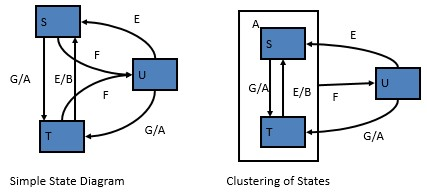
\includegraphics[width=12cm,height=5cm]{Screenshot.jpg}
\caption{Clustering(1)}
\end{figure}\\
Clustering reduces number of transitions in a statechart Expanding state A showing its substates is called as refinement.\\


\subsection{Orthogonality}
In the above section we have seen that the state comprises of two or more states is a superstate.Examples in the above section, the superstate is the OR decomposition of states. In this section we introduce AND decomposition, capturing the property that, being in a state, the system must be in all of its AND components. The notation used in statecharts is the physical splitting of a box into components using dashed lines.\\
\textbf{EXAMPLE:}\\
Figure3 shows a state C consisting of AND components A and B, with the property that being in C entails being in some combination of X,Y,or Z with R or S. We say that C is the orthogonal product of A and B. The components A and B are no different conceptually from any other superstate; they have defaults, internal transitions,etc. Entering C from outside,in the absence of any additional information, is actually entering the combination (X,R) by the default arrow.If event t1 occurs , it transfers X to X itself and Rt to S, resulting in new combine state (X,S). This illustrates a certain kind of synchronization: a single event causing two simultaneous  happenings.\\
\begin{figure}[h]
\centering
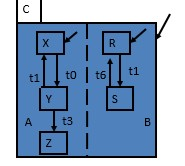
\includegraphics[width=7cm,height=5cm]{Screenshot002.jpg}
\caption{Orthogonality}
\end{figure}\\
\newpage
\subsection{Condition and Selection Entrances}
\textbf{Condition:}\\
Upon the entrance of the superstate a condition is checked and the transition is made to one of the sub-states in the superstate. Here Figure5(b) can replace  Figure5(a).\\ 
\begin{figure}[h]
\centering
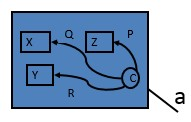
\includegraphics[width=7cm,height=5cm]{Screenshot004.jpg}
\caption{Conditional Entrance}
\end{figure}\\
\textbf{Selection:}\\
The transition is made depending on the generic value of the input rather than the condition.
\begin{figure}[h]
\centering
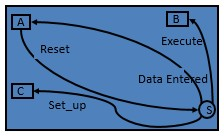
\includegraphics[width=7cm,height=5cm]{Screenshot005.jpg}
\caption{Selection Entrance}
\end{figure}\\
\newpage
\subsection{Delays and Timeouts:}
Sometimes the transition from one state to another occurs precisely when the specified number of time units have elapsed from the occurence of the specified event.\\
\textbf{EXAMPLE:}\\
\begin{figure}[h]
\centering
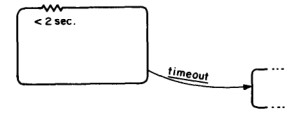
\includegraphics[width=7cm,height=5cm]{timeout.jpg}
\caption{Transition on Timeout}
\end{figure}\\

\subsection{Significance of System's History}
In a multi-superstate system when an event causes transition from one superstate to another,on what basis system will decide the transition to a particular substate of that superstate?. Here is the answer.One of the most interesting  and frequent  ways of entering  a group of states is by the system$^'$s history in that group.  The simplest  kind of this enter-by-history  is entering  the state most recently  visited. Shallow history(H) represents the most recently entered state at the same level. Deep history represents entering the most recently visited state irrespective of how deep the state is. In the following example history chooses between G and F. H remembers between A,B,C,D,E. H remembers the last sub-state the system left. $H^*$-System will enter the most recently visited states.$H^*$ remembers the last sub-state the system left, irrespective of how deep it may be when considered with the history state. B and C are the default initial states for G and F.
\begin{figure}[h]
\centering
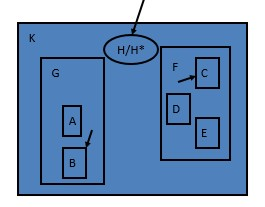
\includegraphics[width=8cm,height=6cm]{Screenshot003.jpg}
\caption{System's History}
\end{figure}\\
\section{Statechart Editor Tools}
The free to use, open source toolkit Statechart Tools (SCT) provides an integrated modeling environment for the specification and development of reactive, event-driven systems based on the concept of statecharts. Many statechart tools are available in the market. These statechart tools contains features like editing,validation,simulation and code generation. The dynamic behaviour of sysytem can be analyse using simulation feature. The code generation feature of statechart tools reduces development time.
\subsection{YAKINDU SCT Software}
This software gives all the features mentioned above. This software is easy to install and all the manuals are available at \href{https://www.itemis.com/en/yakindu/statechart-tools/}{YAKINDU SCT}.\\
This is a typical workspace of YAKINDU SCT.
\begin{figure}[h]
\centering
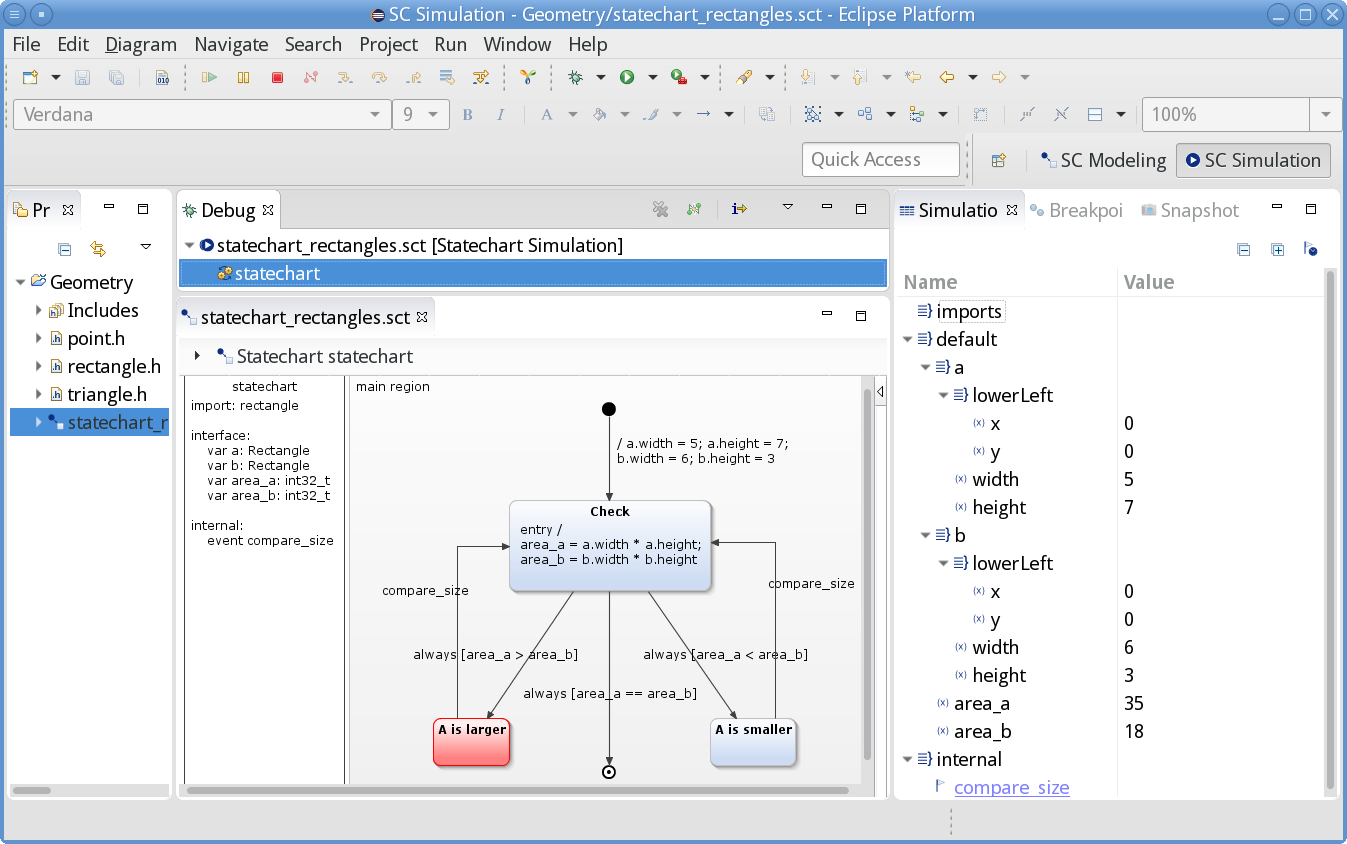
\includegraphics[width=12cm,height=10cm]{gui.png}
\caption{YAKINDU GUI}
\end{figure}\\
\newpage
\subsection{Features of YAKINDU SCT}
\begin{itemize}
\item Editing feature gives an intuitive combination of graphical and textual notation. While states, transitions and state hierarchies are graphical elements, all declarations and actions are specified using a textual notation.\\
\item The validation of state machines includes syntax and semantic checks of the full model.\\
\item The simulation of state machine models allows the dynamic semantics to be checked. Active states are directly highlighted in the statechart editor and a dedicated simulation perspective features access to execution controls, inspection and setting variables, as well as raising events.\\
\item The most important feature of YAKINDU SCT is code generation. SCT includes code generation for JAVA,C AND CPP. Following image shows the code generation feature in YAKINDU SCT\\
\begin{figure}[h]
\centering
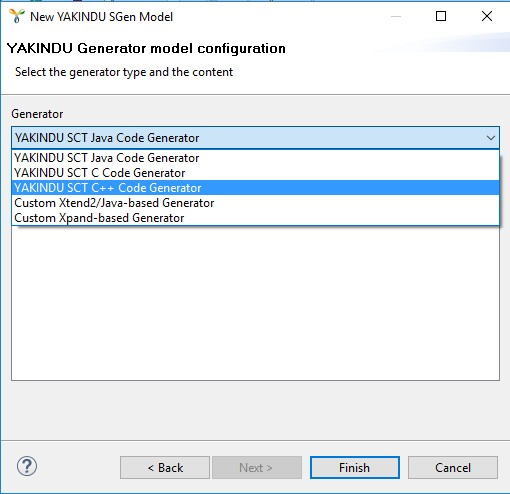
\includegraphics[width=10cm,height=8cm]{code.jpg}
\caption{Code Generation in YAKINU SCT}
\end{figure}
\end{itemize}
\newpage
\subsection{Tasks Modeled}
\begin{enumerate}
    \item Water Level Controller\\
    This is a simple example of water level controller. This system first checks the water level in the tank. If tank is empty then it turns on the motor pump and increment he water level in statechart model when we simulate the model. When water level reaches to peak point it turns off the motor pump.\\
    \begin{figure}[h]
\centering
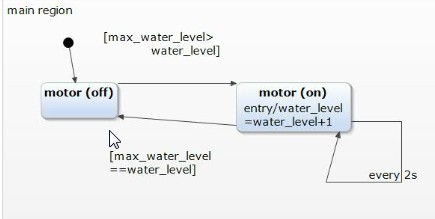
\includegraphics[width=8cm,height=6cm]{Screenshot006.jpg}
\caption{Water Level Controller}
\end{figure}\\
\newpage
\item Real Time Clock\\
This statechart model of real time clock converts time into a single integer value. Using few mathematical syntax we are converting this integer into hours, minutes and seconds to display. We can even set a particular time by generating SET event.\\
\begin{figure}[h]
\centering
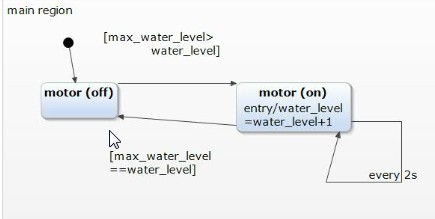
\includegraphics[width=8cm,height=6cm]{Screenshot006.jpg}
\caption{Real Time Clock}
\end{figure}\\
\end{enumerate}

\end{document}